\documentclass[english,usenames,dvipsnames]{beamer}
\usetheme{Boadilla}
\usepackage[utf8]{inputenc}
\definecolor{myred1}{RGB}{255,50,0}
\definecolor{myblue1}{RGB}{0,100,255}
\definecolor{mygreen1}{RGB}{34,139,35}


\title{Should We Allow Non-Competes?}
\author{Nico Fernandez-Arias}
\date[Dec 14 2017]{Macro Workshop, Dec 14, 2017}

\begin{document}
	
\frame{\titlepage}

\begin{frame}{Motivation}
\label{Motivation}
\begin{itemize}
	
	\item A non-compete is a clause in an employment contract preventing the employee from working for a competitor until usually 1-2 years after employment ends
	
	\item Most states in US enforce (at least for knowledge / tech workers and/or "key employees") 
	
	\item Prevalent among innovative workers
	\begin{itemize}
		\item 70\% of senior executives (Garmaise 2011)
		\item Nearly 50\% of engineers (Marx 2011)
	\end{itemize}

\end{itemize}
\end{frame}

\begin{frame}{Motivation - Policy issue}
\begin{itemize}
	\item Economic literature has tentatively endorsed the view that Silicon Valley, CA displaced Rt. 128, MA as
	high-tech hub due to non-enforcement (Saxenian 1994, Gilson 1999, etc.)
	\item Policymakers converging to belief that not enforcing is key to creating high-tech hub
	\begin{itemize}
		\item 2015 - Hawaii passes law precluding enforcement of non-competes for "technology workers"
		\item Several states considering weakening enforcement explicitly in an effort to imitate California \hyperlink{mapofenforcement}{\beamerbutton{map}} 
		\item Oct 2016: Obama administration report, ``call to action'' to state legislatures
		to reduce enforcement of non-competes
		\begin{itemize}
			\item Mostly about requiring informing about non-compete requirement and banning non-competes for low-wage workers (e.g. cafeteria workers) 
		\end{itemize}
	\end{itemize}
\end{itemize}
\end{frame}

\begin{frame}{Motivation - Tradeoffs}
\begin{itemize}
	
	\small
	\item Non-competes...
	\begin{itemize}
		\footnotesize
		\item Protect intellectual property (Sometimes can't patent, non-disclosure agreements hard to enforce)
		\item Prevent knowledge diffusion (reduce production possibilities of the economy)
		\item Increase employer incentive to invest in worker human capital
		\item Reduce employee incentive to invest in own human capital 
		\item Reduce worker bargaining power
		\item Prevent workers hopping jobs until find a good match
		\item Harm reallocation after layoffs
		\item May lead to more market concentration
	\end{itemize}

	\small
	\item But...freedom of contract inefficient? 
	\begin{itemize}
		\footnotesize
		\item No welfare theorems here..so there may be externalities
		\item Burden of proof still on those who say freedom of contract is inefficient...
		\item In particular since many criticisms \textbf{hurt parties to the contract} (key difference to patents)
	\end{itemize}

\end{itemize}
\end{frame}

\begin{frame}{Existing empirical work}
\begin{itemize}
	\item In non-enforcing regimes:
	\begin{itemize}
		\item Employment / payroll / business formation grows more in response to exogenous increases in the supply of VC funding (Samila-Sorenson 2011)
		\item More workforce mobility (Fallick et al. 2006, Garmaise 2011, Marx et. al 2009)
		\item Less market concentration (Kang-Fleming 2017)
		\item Employees have better lifetime wage profiles (Chang et al. 2017)
	\end{itemize}
	\item Knowledge spillovers contribute 20\% of productivity growth in IT sector (Tambe-Hitt 2014)
\end{itemize}
\end{frame}

\begin{frame}{Existing empirical work (cont.)}
\begin{itemize}	
	\item Existing work cannot identify aggregate effect if non-enforcing states crowd out enforcing states
	\begin{itemize}
		\item Analogous to inability to identify aggregate effect of shocks in Autor-Dorn-Hanson 2013 and similar papers	
	\end{itemize}
	\item Direct evidence of crowding out: brain drain from enforcing to non-enforcing (Marx 2015)	
\end{itemize}
\end{frame}

\begin{frame}{Existing theoretical work}
\begin{itemize}
	\item Some work exists...
	\begin{itemize}
		\item Franco-Filson 2006 
		\item Shankar-Ghosh 2013
		\item Shi 2017
	\end{itemize}
	\item But shortcomings...
	\begin{itemize}
		\item No creative destruction $\rightarrow$ misleading Pareto efficiency results	
		\item No long-run growth (2- or 3-period models), so not GE in dynamic sense --> bad for model of endogenous growth
		\item Focus on managerial labor market --> not the key labor market 
	\end{itemize}
\end{itemize}
\end{frame}

\begin{frame}{Proposal}
\begin{itemize}
	\item Write a structural model of R\&D-driven productivity growth 
	\begin{itemize}
		\item E.g., high-tech industry like biotech, computer hardware, artificial intelligence, etc.
		\item Endogenous knowledge spillovers from employees spinning out firms (which compete in R\&D race)
		\item Creative destruction
		\item Enforcing \& non-enforcing regions
	\end{itemize}
	\item Calibrate / test with micro data / existing empirical work (e.g. cross-sectional results, brain drain)
	\begin{itemize}
		\item LEHD probably won't work
		\item "New" data: Crunchbase
		\item Maybe replace LEHD withu LinkedIn data, but not very optimistic - hard to scrape (could ask, but doubt I will get access)
	\end{itemize}
	\item Use model to assess effect of non-competes on productivity growth and welfare
\end{itemize}
\end{frame}

\section{Data}
\begin{frame}{Data}
\begin{itemize}
	\item Crunchbase (have obtained)
	\begin{itemize}
		\item Employer-employee matched data
		\item Coverage: mostly startups 
		\item Worldwide, but US coverage better
		\item Information on founders and some C-level employees and board members, funding rounds 
	\end{itemize}
	\item LinkedIn possibly
	\begin{itemize}
		\item Previous occupation of firm founders
	\end{itemize}

	\item LEHD (US Census)
	\begin{itemize}
		\item Plan was to use these data to (1) improve observation of process of employees starting / joining competing startups / firms, and (2) get wage distributions to match 
		\item California and Massachusetts never approve
		\item In addition, would need significant funding (\$25,000) to merge datasets by employee name 
	\end{itemize}
\end{itemize}
\end{frame}

\section{Model}
\subsection{Overview}
\begin{frame}{Model: Workers}
\begin{itemize}
	\item Unit mass continuum of risk-neutral individuals indexed by $i\in I =[0,1]$, with objective
	\begin{align*}
		U = \int_0^{\infty}\exp(-\rho t)c(t)dt
	\end{align*}
	where $c(t)$ is final goods consumption at $t$.
	\item Individuals can supply labor to final goods production ($l^F$), intermediate good production ($l^I$) and R\&D ($l^{RD}$) such that 
	\begin{align*}
		l_t^F+ l_t^I + l_t^{RD} = 1
	\end{align*}
	\item Aggregate labor market satisfies (where $L_t^k = \int_I l_t^k(i)di$)
	\begin{align*}
		L_t^F + L_t^I + L_t^{RD} = 1
	\end{align*}
\end{itemize}
\end{frame}

\begin{frame}{Model: Intermediate goods production}
\begin{itemize}
	\item Continuum of intermediate goods, indexed by $j\in J = [0,1]$
	\item Denote quality of good $j$ by $q_j$, amount produced by $k_j$
	\item Each good produced with technology 
	\begin{align*}
	k_j = \overline{q} l_j
	\end{align*}
	where $\overline{q} = \int_0^1 q_j dj$ is the average quality level of the economy
	\item Alternative setup 
	\begin{align*}
	k_j = q_j l_j
	\end{align*} 
	requires slightly modified final goods production function
	
\end{itemize}
\end{frame}

\begin{frame}{Model: Final good production}
\begin{itemize}
	\item Final good is produced using labor and a continuum of intermediate goods $j\in[0,1]$ with production technology
	\begin{align*}
	Y(t) &= (1-\beta)^{-1} L(t)^{\beta}\Bigg(\Big(\int_0^1 q_j(t)^\beta 
	k_j^{1-\beta}(t)dj \Big)^{1/(1-\beta)}\Bigg)^{1-\beta} \\
		&= (1-\beta)^{-1} L(t)^{\beta}\int_0^1 q_j(t)^\beta k_j^{1-\beta}(t)dj
	\end{align*}
	where $q_j$ is quality, $k_j$ is quantity
	\item Restricts labor share to be related to markup $\mu = 1/(1-\beta)$ but necessary for BGP
	\item There may be a way to relax this using Oberfield et. al "Balanced Growth Despite Uzawa"
\end{itemize}
\end{frame}

\subsection{R\&D and knowledge spillovers}
\begin{frame}{Model: R\&D overview}
\begin{itemize}
	\item R\&D improves quality of intermediate goods, generates long-run growth
	\item Incumbent has monopoly on good $j$ production
	\item Incumbent initially has monopoly on good $j$ R\&D
	\item R\&D "spills" knowledge to R\&D employees who become entrants after non-competes expire 
	\item Incumbent and entrants perform R\&D to improve quality to $(1+\lambda) q_j$
	\item Upon discovery, become incumbent with monopoly
\end{itemize}
\end{frame}

\begin{frame}{Model: R\&D technology}
\begin{itemize}
	\item $z$ units of labor yields innovations at Poisson rate
	\begin{align*}
	R_I(z_I;\overline{z}) &= \chi_I z_I \phi(\overline{z}) \\
	R_E(z_E;\overline{z}) &= \chi_E z_E \phi(\overline{z}) 
	\end{align*}
	where 
	\begin{align*}
	\overline{z} = \int_0^m z(\ell)d\ell + z_I
	\end{align*}
	is total innovation effort on $j$, with (endogenous) mass $m$ of entrants indexed by $\ell$.
	\item $\phi(z)$ decreasing, $z\phi(z)$ increasing
	\item Entrant $\ell$ can hire $z\le\xi$ units of R\&D labor (in equilibrium $z(\ell) = \xi$)
\end{itemize}
\end{frame}

\begin{frame}{Model: R\&D spillovers}
\begin{itemize}
	\item Individual supplying R\&D labor to an intermediate goods firm (or entrant) acquires the knowledge required to enter the race at rate $\nu$ per unit of labor
	\item At Poisson rate $v$, these workers transition out of competition-restricted status ("Perpetual youth": tractability)
	\item $n_j$ is mass of workers with knowledge who are still bound by non-competes; $m_j$ is those whose non-competes expired 
	\item Laws of motion
	\begin{align*}
	\dot{n}_j &= \nu l_j^{RD} - vn_j \\
	\dot{m}_j &= vn_j
	\end{align*}
	\item Note that $(q_j,m_j,n_j)$ is the state of product $j$	
\end{itemize}
\end{frame}

\begin{frame}{Model: R\&D spillovers}
\begin{table}
	\begin{tabular}{p{0.8\textwidth}}
		\centering
		Participant in the R\&D race for good $j$ begins with monopoly on good $j$ R\&D \\
		 $\downarrow$\\
		Hires R\&D labor; at rate $\nu$ per unit of R\&D labor hired, an employee acquires knowledge to open rival R\&D lab (but not to compete directly on product market). \\
		$\downarrow$\\
		This worker becomes part of mass $n_j$ and leaves the lab (replaced by someone who wants the knowledge)\\ 
		$\downarrow$\\
		At rate $v$, agents' non-competes expire, adding to the mass $m_j$ \\
		$\downarrow$\\
		At some point, either incumbent or entrant wins patent race, restarting the process 
	\end{tabular}
\end{table}
\end{frame}

\subsection{Optimization}
\begin{frame}{Final goods production}
	\begin{align*}
Y(t) &= (1-\beta)^{-1} L(t)^{\beta}\Bigg(\Big(\int_0^1 q_j(t)^\beta 
k_j^{1-\beta}(t)dj \Big)^{1/(1-\beta)}\Bigg)^{1-\beta}
\end{align*}
\begin{itemize}
	\item CRS implies no profits
	\item CES implies constant markups $\mu = (1-\beta)^{-1}$ in equilibrium
	\item Closed form solution for final goods wage  $\overline{w}_t = \beta^{\beta}(1-\beta)^{1-2\beta} \overline{q}_t$
\end{itemize}
\end{frame}

\begin{frame}{Worker optimization}
\small
\begin{itemize}
	\item Workers indifferent between occupations (Final goods, intermediate goods, R\&D)
	\item Final goods wage pinned down by $\overline{q}_t$ at $\overline{w}_t = \beta^{\beta}(1-\beta)^{1-2\beta} \overline{q}_t$
	\item Intermediate goods wage $w^I_t = \overline{w}_t$ 
	\item R\&D wage at product $j$ depends on state of the product, which is $(q,m,n)$
	\item Indifference condition
	\begin{align*}
	w_t(q,m,n) + \nu W^{NC}_t(q,m,n) &= \overline{w}_t
	\end{align*}
	where $W^{NC}_t(q,m,n)$ is the value of the knowledge (bound by a non-compete)
	\item Since $w_t(q,m,n) < \overline{w}_t$, workers will switch to a different R\&D employer once they attain knowledge (workers are infinitesimal so this goes on forever)
\end{itemize}
\end{frame}

\begin{frame}{Worker optimization timeline}
\begin{table}
	\begin{tabular}{p{0.8\textwidth}}
		\centering
		Allocates labor to R\&D and final and intermediate good production \\
		 $\downarrow$\\
		While performing R\&D for good $j$ hit by knowledge shock with intensity $\nu$ per unit of R\&D labor supplied to $j$ \\
		$\downarrow$\\
		No longer works for good $j$ until next step on ladder (because already has knowledge) \\
		$\downarrow$\\
		When hit by non-compete expiry shock, and provided $m<M(q)$ threshold mass of entrants, hires $\xi$ units of R\&D labor and enters R\&D race (continue to work throughout -- no worker / entrepreneurship choice)
	\end{tabular}
\end{table}
\end{frame}


\begin{frame}{Intermediate goods firms optimization}
\begin{itemize}
	\small
	\item Making the environment stationary: let $\tilde{q}$ denote $qe^{-gt}$ where $g$ is growth rate on BGP 
	\item Value function of \textbf{incumbent} $A_t(q,m,n) = e^{gt}A(\tilde{q},m,n)$

	\item CES demand structure implies constant markup over marginal cost, flow profit function $\pi(\tilde{q}) = \tilde{\pi}\tilde{q}$ in eq.
	\item HJB:
	\footnotesize
	\begin{align*}
	(\rho - g)A(\tilde{q},m,n) &= \pi(\tilde{q}) - g\tilde{q}A_{\tilde{q}}(\tilde{q},m,n) \\
							   & + \max_{\textcolor{myred1}{z}} \Big\{\chi_I\textcolor{myred1}{z}\phi(\textcolor{myred1}{z}+ \textcolor{mygreen1}{\overline{z}_E(\tilde{q},m,n)})\overbrace{\textcolor{myblue1}{\Big(A((1+\lambda)\tilde{q},0,0)-A(\tilde{q},m,n)\Big)}}^{\text{NPV of successful innovation}} \\
							   & - w(\tilde{q},m,n)\textcolor{myred1}{z} +(\nu(\textcolor{myred1}{z}+\textcolor{mygreen1}{\overline{z}_E(\tilde{q},m,n)})-vn)A_n(\tilde{q},m,n) \\
							   & +vnA_m(\tilde{q},m,n) - \textcolor{mygreen1}{\chi_E\overline{z}_E(\tilde{q},m,n)}\phi(\textcolor{myred1}{z}+\textcolor{mygreen1}{\overline{z}_E(\tilde{q},m,n)})\Big\} 
	\end{align*}
	\normalsize
	\item $A_m,A_n<0$ and $A_{\tilde{q}} > 0$ 
\end{itemize}
\end{frame}

\begin{frame}{Intermediate goods firms optimization (cont.)}
\begin{itemize}
	\small
	\item Value function of \textbf{entrant no longer bound by non-compete} is $W^{F}(\tilde{q},m,n)$
	\item HJB:
	\footnotesize
	\begin{align*}
	(\rho - g)W^F(\tilde{q},m,n) &= - g\tilde{q}W^F_{\tilde{q}}(\tilde{q},m,n) \\
	& + \max_{\textcolor{myred1}{z}} \Big\{\chi_E\textcolor{myred1}{z}\textcolor{mygreen1}{\phi(\overline{z}(\tilde{q},m,n))}\overbrace{\textcolor{myblue1}{\Big(A((1+\lambda)\tilde{q},0,0)-W^F(\tilde{q},m,n)\Big)}}^{\text{NPV of successful innovation}} \\
	& - w(\tilde{q},m,n)\textcolor{myred1}{z} +(\nu \textcolor{mygreen1}{\overline{z}(\tilde{q},m,n)}-vn)W^F_n(\tilde{q},m,n)+vnW^F_m(\tilde{q},m,n) \\
	& - \textcolor{mygreen1}{(\chi_Iz_I(\tilde{q},m,n)+\chi_E\overline{z}_E(\tilde{q},m,n)\phi(\overline{z}(\tilde{q},m,n))}W^F(\tilde{q},m,n)\Big\} 
	\end{align*}
	\small
	\item $W^F_m,W^F_n<0$ and $W^F_{\tilde{q}} > 0$ 
	\item Entrants continue to enter until a mass $m = M(\tilde{q})$, defined as the mass of entrants if we assumed (1) free entry and (2) each hires $\xi$ units of R\&D labor
	\item Hence total policy will be $\overline{z}_E(\tilde{q},m,n) = \xi \min (M(\tilde{q}),m)$
\end{itemize}
\end{frame}

\subsection{Equilibrium}
\begin{frame}{Equilibrium}
\small
\begin{itemize}
	\item An equilibrium consists of: growth rate $g$, value functions $A(\tilde{q},m,n),W^F(\tilde{q},m,n) and W^NC(\tilde{q},m,n)$, R\&D wages $w(\tilde{q},m,)$, production wage $\overline{w}$, prices and quantities of intermediate goods, research effort policies $z_I(\tilde{q},m,n)$ and $z_E(\tilde{q},m,n)$, and production labor allocations $L^F$ and $L^I(j)$ such that:
	\begin{itemize}
		\item Value functions solve HJBs (with relevant boundary conditions)
		\item Research effort policies are optimal
		\item R\&D wages satisfy indifference condition $w(\tilde(q,m,n)) + \nu W^{NC}(\tilde{q},m,n) = \overline{w}$
		\item Final goods firms and intermediate goods firms optimize production, pricing and demand for intermediate goods and labor
		\item etc.
	\end{itemize} 
\end{itemize}
\end{frame}

\section{Extensions}
\begin{frame}{Possible extensions or improvements}
\begin{itemize}
	\item Add mechanisms
	\begin{itemize}
		\item Incentives for worker \& firm investment into human capital
		\item Reallocation of workers across firms 
	\end{itemize}
	\item Enforcing and non-enforcing regions
	\begin{itemize}
		\item Test if model can reproduce cross-sectional results (e.g. brain drain)
		\item Geography
	\end{itemize}
	\item When are non-competes used in enforcing regions?
	\begin{itemize}
		\item E.g., non-competes that harm parties relative to no non-compete shouldn't be signed in equilibrium
		\item Assuming all are signed / all are same could exaggerate case against non-competes
	\end{itemize}
\end{itemize}
\end{frame}


\begin{frame}{Enforcement}\label{mapofenforcement}
\hyperlink{Motivation}{\beamerbutton{back}}

\begin{figure}
	\caption{Map of enforcement across US states (for technology workers)}
	
	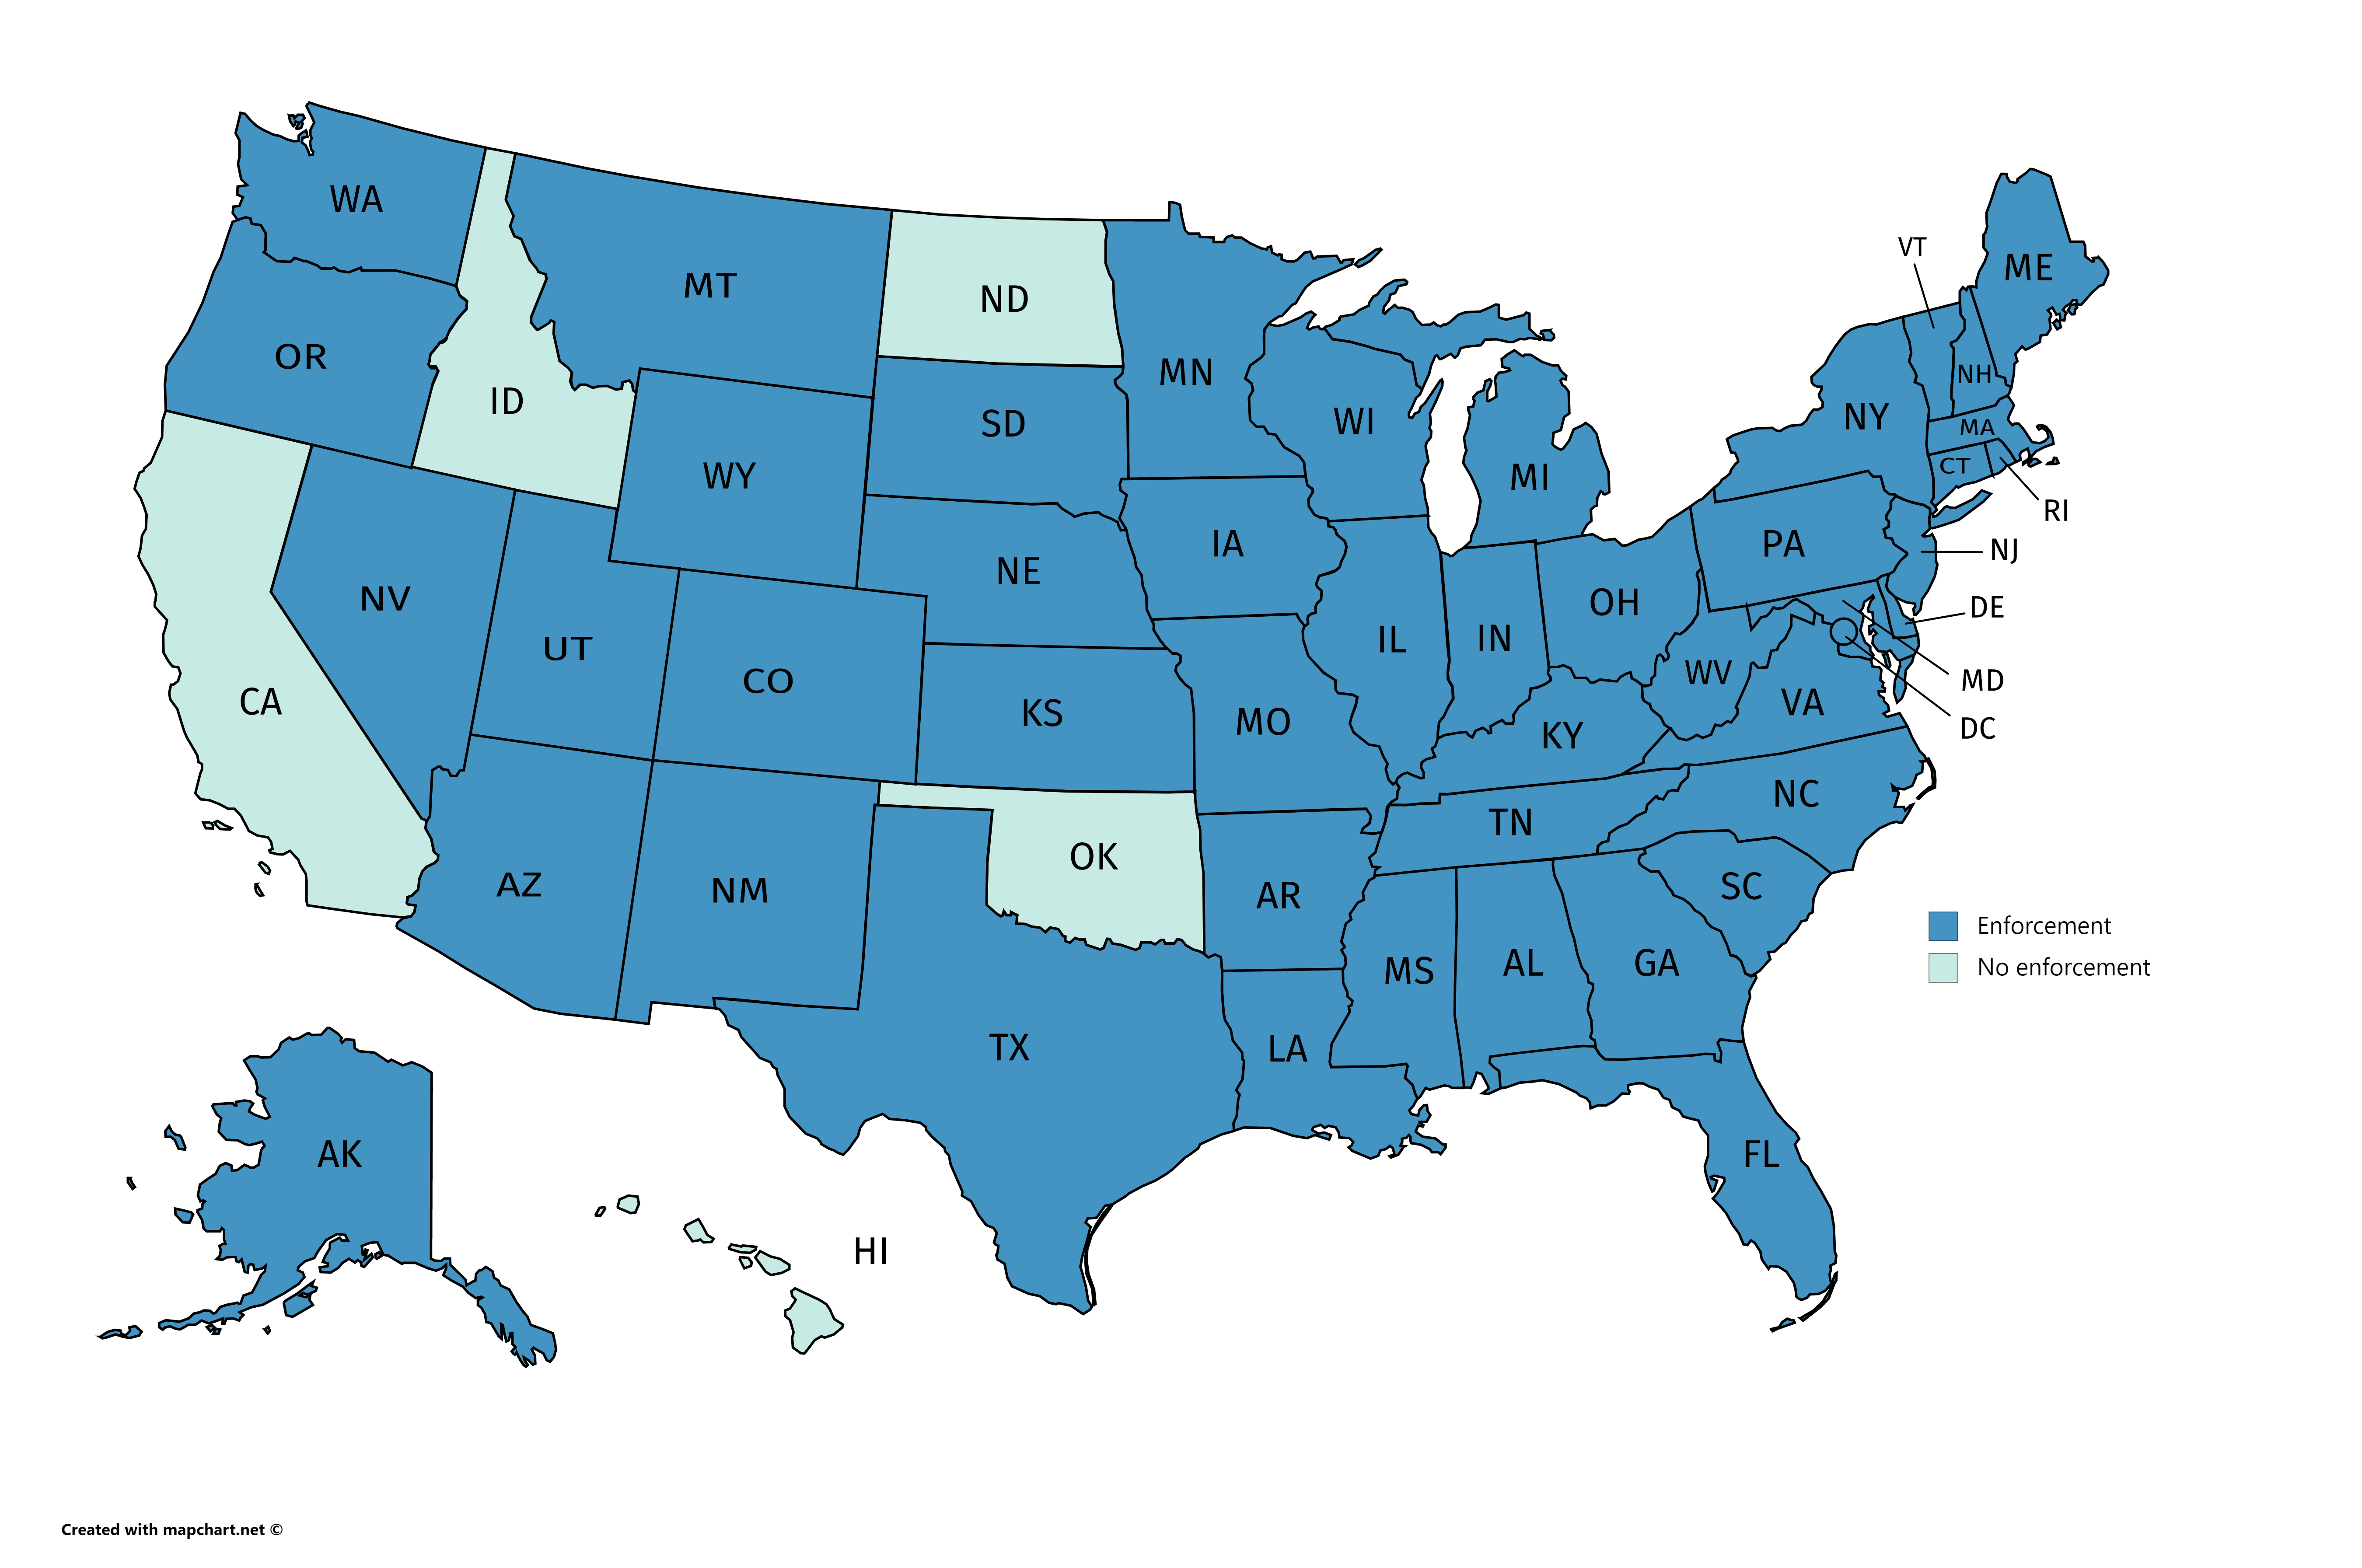
\includegraphics[scale=0.05]{figures/map_of_enforcement}
	
\end{figure}
\end{frame}







\end{document}